% musicar EuroHPC Development Access application text.
% Build from this folder: pdflatex musicar_eurohpc_dev_outline.tex (twice). Working notes: context/claude/musicar_eurohpc_working_notes.md (git-ignored).
\documentclass[11pt,a4paper]{article}
\usepackage[T1]{fontenc}
\usepackage[utf8]{inputenc}
\usepackage{lmodern}
\usepackage[margin=2.5cm]{geometry}
\usepackage{xcolor}
\usepackage{enumitem}
\usepackage{array}
\usepackage{tabularx}
\usepackage{longtable}
\usepackage{amsmath}
\usepackage{amssymb}
\usepackage{graphicx}
\usepackage[hidelinks]{hyperref}
\usepackage{url}
% visible links in Section 1 only (the rest of the document keeps hidelinks)
\newcounter{refc}
\newcommand{\seclink}[2]{\hyperref[#1]{\textcolor{blue!60!black}{\underline{#2}}}}
\newcommand{\weblink}[2]{\href{#1}{\textcolor{blue!60!black}{\underline{#2}}}}
\makeatletter\g@addto@macro\UrlBreaks{\do\_\do-}\makeatother

\definecolor{head}{RGB}{25,85,140}
\makeatletter
\renewcommand\section{\@startsection{section}{1}{\z@}{-3.2ex \@plus -1ex \@minus -.2ex}{1.8ex \@plus .2ex}%
  {\normalfont\Large\bfseries\color{head}}}
\renewcommand\subsection{\@startsection{subsection}{2}{\z@}{-2.6ex \@plus -1ex \@minus -.2ex}{1.2ex \@plus .2ex}%
  {\normalfont\large\bfseries\color{head}}}
\renewcommand\subsubsection{\@startsection{subsubsection}{3}{\z@}{-2.2ex \@plus -.5ex \@minus -.2ex}{0.8ex \@plus .2ex}%
  {\normalfont\normalsize\bfseries\color{head}}}
\def\ps@outline{%
  \def\@oddhead{\vbox{\hbox to\textwidth{\small musicar -- EuroHPC Development Access\hfil Application text}%
    \vskip 3pt\hrule height 0.4pt}}%
  \let\@evenhead\@oddhead
  \def\@oddfoot{\hfil\small\thepage\hfil}\let\@evenfoot\@oddfoot}
\makeatother
\pagestyle{outline}
\renewcommand{\contentsname}{\color{head}Contents}
\setlist[itemize]{label=--,nosep,leftmargin=1.2em}
\setlength{\parindent}{0pt}
\setlength{\parskip}{3pt}
\newcommand{\mk}[1]{[\textbf{#1}]}
\renewcommand{\arraystretch}{1.15}
\newcolumntype{L}[1]{>{\raggedright\arraybackslash}p{#1}}
% \slot[lines]: empty framed box for the author's own text
\newcommand{\slot}[1][4]{\par\smallskip\noindent\fbox{\parbox[t][#1\baselineskip][t]{\dimexpr\linewidth-2\fboxsep-2\fboxrule\relax}{\footnotesize\color{gray}Your text}}\par\medskip}

\begin{document}
\thispagestyle{outline}

\begin{center}
{\LARGE\bfseries Scaling a symbolic music model to 1--2B parameters:\\ multi-GPU training development\par}
\vspace{6pt}
{\large EuroHPC JU Development Access application\par}
\vspace{3pt}

%{\small Working draft: section plan only, no body text yet. Updated 22 Nov 2026 with the RTX 5090 scaling
%results.\par} %needs to be removed when I am done with the text

\end{center}
\vspace{6pt}

\begin{tabularx}{\textwidth}{|L{3.9cm}|X|}
\hline
Principal investigator & Dr. Tara Ghasempouri, Tallinn University of Technology (TalTech)\\ \hline
Team member & Dmytro Hilei, TalTech (bachelor student): development, runs, evaluation, writing\\ \hline
Call & EuroHPC JU Call for Proposals for Development Access\\ \hline
Allocation length & 6 months, from about 15 December 2026\\ \hline
System & MareNostrum 5 ACC, BSC (Spain): 4$\times$ NVIDIA H100 64 GB per node\\ \hline
Request & 1,780--2,500 H100 hours (445--630 node hours)\\ \hline
\end{tabularx}
\vspace{4pt}

\vspace{6pt}
\tableofcontents

\section{Project}\label{sec:project}

\subsection{Title}
Scaling a symbolic music model to 1--2B parameters: multi-GPU training development

\subsection{Summary}

\textbf{What exists}
\begin{itemize}
\item \textbf{musicar-L}: 464M parameters, trained from scratch on \textbf{one rented RTX 5090 in about 41 h}.
\item Weights, code and evaluations are public:
\weblink{https://github.com/DmytroHilei/Music_generative_model}{GitHub},
\weblink{https://huggingface.co/Dimitri-206265/musicar-L}{musicar-L on Hugging Face},
\weblink{https://huggingface.co/Dimitri-206265}{all models}.
\item \textbf{Continuation}: on 96 continuation prompts, CLaMP 3 rates musicar-L's continuations closer to the real
ones than those of AMT large (780M) and SkyTNT medium (234M) in all 10,000 paired draws (closeness 0.715 vs 0.648
for both, first 1,000 new notes; also over 200). On the distance D (density and instrument use), AMT and musicar-L are
too close to rank.
\end{itemize}

\medskip
\textbf{What the project develops}
\begin{itemize}
\item The single-GPU trainer turned into a \textbf{multi-GPU trainer on 4$\times$H100 nodes}: data parallel, FP8,
NorMuon at scale. Multi-node and sharding come after the paper runs.
\end{itemize}

\medskip
\textbf{What it tests}
\begin{itemize}
\item \textbf{How well large MIDI models scale}: whether the loss of the 1B and 2B runs (2B: 37 transformer blocks of
width 2112; 2.03B parameters in total, of which 1.98B in the blocks) follows the \textbf{scaling law fitted to a study of about 200 single-GPU runs}, with the predictions committed
before the runs.
\item \textbf{How much repeated data costs at these sizes}: the open MIDI corpora we collected hold 8.84B unique notes, so the 2B run
sees each note about 5--6 times. The runs measure the loss gap to all-new data (predicted 0.001 and 0.004 nats,
against 0.029 between the 1B and 2B forecasts).
\item \textbf{Whether lower loss gives better music}: each run against musicar-L and the open baselines on
continuation and caption tests, and in a blind listening test.
\item \textbf{How to make music models follow captions over long pieces}: a stronger trained text encoder and a
16,384-note context, tested at 1B after the main runs. We know of no published answer yet.
\item \textbf{The training method itself}: the multi-GPU trainer at 1B and 2B; 2.5B as an option.
\end{itemize}
Background and evidence: \seclink{sec:gap}{Section~\ref*{sec:gap}} (gaps) and
\seclink{sec:prelim}{Section~\ref*{sec:prelim}} (scaling study).

\medskip
\textbf{What comes back}
\begin{itemize}
\item Open weights, code and logs; the forecast against the measured loss; a write-up acknowledging EuroHPC.
\item To our knowledge \textbf{the largest open model trained only on MIDI}, and a measured repetition cost that lets
later work scale MIDI models further on the same data (\seclink{sec:gap}{Section~\ref*{sec:gap}}).
\end{itemize}

\medskip
\textbf{Why EuroHPC}
\begin{itemize}
\item On one RTX 5090 at musicar-L's measured compute rate ($2.3\times10^{19}$ FLOP in 41 h), the 2B run (41--55B notes) would take \textbf{5--7 weeks}
and the 1B run 9--11 days.
\item On one 4$\times$H100 node, both runs take \textbf{7--9 days} at the rates measured on an H100 (scaled to the 2B shape).
\item Total request: \textbf{1,780--2,500 H100 hours}
(\seclink{sec:resources}{Section~\ref*{sec:resources}}).
\end{itemize}

\subsection{Keywords}

\noindent Symbolic music generation, MIDI, generative AI, text-conditioned music generation, decoder-only
transformer, scaling laws, compute-optimal training, data repetition, distributed data-parallel training, FP8 mixed
precision, Muon optimizer, NVIDIA H100, open weights

\subsection{Research fields and submission details}

\begin{itemize}
\item \textbf{Research field}: PE6 Computer Science and Informatics, 100\%.
\item \textbf{AI technologies}: Deep Learning; Generative Language Modeling (musicar is a language model over notes).
\item \textbf{Preferred starting date}: 15 December 2026.
\item \textbf{Industry involvement}: none. \textbf{Public sector involvement}: none.
\item \textbf{Civilian purpose}: yes. \textbf{Confidential part}: no (weights, code and logs are released).
\end{itemize}

\subsection{Project duration}
\begin{itemize}
\item \textbf{6 months}: about 15 December 2026 to mid-June 2027.
\item The main runs fill the first 3 months (trainer on 4 GPUs by about 10 January, the 1B run by about 21 January, the 2B run by
early February, evaluation in February). Months 4--6 hold the ablations, the optional 2.5B run, queue waits and the
release; the paper draft is due in March for ISMIR 2027.
\item Final report by mid-September 2027 (3 months after the end).
\item The PI holds a permanent contract at TalTech, so the contract runs well past the final report.
\end{itemize}

\section{Principal investigator and team}\label{sec:pi}
\begin{itemize}
\item \textbf{Principal investigator}: Dr. Tara Ghasempouri, Tallinn University of Technology (TalTech), Estonia.
Submits the proposal on behalf of the group, accepts the award and submits the final report.
\item \textbf{Team member}: Dmytro Hilei, bachelor student at TalTech. Author of musicar: model, trainer, data
pipeline, scaling study and evaluation, all public on GitHub and Hugging Face. Does the development, the runs, the
evaluation and the writing.
\end{itemize}

\section{Background and objectives}\label{sec:background}

\subsection{Current model and results}\label{sec:current}

\textbf{Model}
\begin{itemize}
\item \textbf{musicar} is a decoder-only transformer over MIDI: \textbf{one compound token per note} (pitch,
velocity, duration and time shift on a 20 ms grid), 129 instruments (128 General MIDI programs and drums), context
2,048 notes. Cascade output heads pick the time shift, instrument, pitch, duration and velocity of the next note
one after another, each seeing the values already chosen.
\item \textbf{musicar-L}: 464M parameters (28 blocks, width 1152), Muon and AdamW, bf16 with FP8 matrix multiplies.
\item Trained from scratch on \textbf{8.3B notes} (GigaMIDI, Aria-MIDI and a Discover MIDI subset; about 1.8 passes) on
\textbf{one rented RTX 5090 in about 41 h} ($2.3\times10^{19}$ FLOP, about 56k notes/s). Held-out loss 1.641 nats per
note on the scaling study's GigaMIDI windows (1.679 on clean GigaMIDI validation, the figure on the model card).
\item \textbf{musicar-L-caption}: musicar-L fine-tuned on 2.18B notes in three stages (main stage 2.04B notes, about 14 h on one RTX 5090) with a frozen multilingual text
encoder (LaBSE), so it takes text prompts in English and Ukrainian.
\weblink{https://huggingface.co/Dimitri-206265/musicar-L-caption}{Hugging Face}, 252 downloads last month (23 Nov).
\end{itemize}

\medskip
\textbf{Results against open models}
\begin{itemize}
\item \textbf{Caption following} on our 28 short prompts (15 English, 12 Ukrainian, 16 pieces each): follow score F
1.07 / 0.95 (English / Ukrainian) for musicar-L-caption against 0.60 / 0.09 for MIDI-LLM (1.72B) and 0.54 / 0.06 for
Text2midi; with a caption-picked real opening, F rises to 1.08 / 1.15. It is the only one of the three that follows
Ukrainian prompts.
\item \textbf{Solo piano} (96 prompts): closer to the real note rate than Aria (D 0.035 vs 0.074). CLaMP 3 puts musicar-L
ahead on closeness over 1,000 notes (0.689 vs 0.658), level on contrast, and Aria ahead over the first 200 notes.
\end{itemize}

\medskip
\textbf{Limits}
\begin{itemize}
\item On the distance D (density and instrument use), AMT and musicar-L are too close to rank (0.097 vs 0.144 on 96 prompts; the order
changes between prompt sets).
\item On 495 long MidiCaps test captions, musicar-L-caption is last on tempo, key, caption match and CLaMP 3; its exact-key match is at the shuffled baseline. Both
rivals were trained on MidiCaps-style captions.
\item The continuation prompts come from GigaMIDI validation, the same corpus family as the training data.
\end{itemize}

\subsection{Gap and motivation}\label{sec:gap}

\textbf{No scaling study for multi-instrument MIDI}
\begin{itemize}
\item Open MIDI models stop below 1B parameters: AMT 780M, Moonbeam 839M, Aria about 0.7B. Text and audio models have
published scaling laws. The one for symbolic music, MuPT (ICLR 2025), is for ABC notation, a text score format,
with models up to about 2B parameters and a term for repeated epochs. Note-level, multi-instrument MIDI has none.
\item Without such a law, the model size and the amount of data for a large run are guesses. Our earlier forecast from
short runs predicted 2.23 nats per note for musicar-L; the measured value is 1.641.
\end{itemize}

\medskip
\textbf{Music data is limited, so large models have to repeat it}
\begin{itemize}
\item The open MIDI corpora we collected hold \textbf{8.84B unique notes} after near-duplicate removal (measured on 23
Nov). Large text models are trained on trillions of tokens.
\item A compute-optimal 2B run needs 41--55B notes, so it sees every note about 5--6 times. The cost of that repetition
is the gap in held-out loss to the same run trained on the same number of all-new notes. At 1--2B parameters this
gap is not known for MIDI and can only be measured at that size.
\end{itemize}

\medskip
\textbf{Lower loss and better music}
\begin{itemize}
\item Scaling laws predict the loss, but listeners hear the music. Our own metrics do not always agree: on solo piano,
CLaMP 3 and the density distance D rank the models differently. Whether a lower loss at 1--2B gives clearly better
continuations and caption following is open.
\end{itemize}

\medskip
\textbf{Why now}
\begin{itemize}
\item A first scaling study for MIDI now exists: about 200 runs on one rented RTX 5090
(\seclink{sec:prelim}{Section~\ref*{sec:prelim}}). Its law predicts musicar-L within 0.02 nats (1.62 vs 1.641),
77$\times$ beyond the largest fitted compute. The 1B and 2B runs test it another 5--22$\times$ further, with the
predictions committed to the public repository before the runs.
\item To our knowledge there is no open, EU-built multi-instrument MIDI model with text prompts at this scale. The
closest European work is at Queen Mary University of London (UK).
\end{itemize}

\medskip
\textbf{What this opens}
\begin{itemize}
\item The 2B run would be, to our knowledge, \textbf{the largest open model trained only on MIDI}.
AMT has 780M parameters and Moonbeam 839M; MIDI-LLM (1.72B) is a text model, Llama 3.2 1B, with MIDI tokens added.
Models on ABC text notation are larger (MuPT, ChatMusician), but they do not model played, multi-instrument MIDI.
\item With the cost of repetition measured at 1--2B, later work can plan larger MIDI models on the same limited data:
how many passes are safe and which size the data supports. This is the route to better music generation beyond
this project.
\end{itemize}

\subsection{Preliminary results: scaling study on one RTX 5090}\label{sec:prelim}
To plan the large runs, we ran a scaling study on one rented RTX 5090 from 20 to 22 November 2026: about 200 runs
of 3M--217M parameters (171 on repetition and augmentation, 35 iso-FLOP), about 40 GPU-hours for about \$23. All
losses are held-out GigaMIDI cross-entropy in nats per note, summed over the four note attributes. The predictions were committed to the public repository
before the confirmatory runs (rows already visible at commit time are marked in the file); the last table of this section lists them against the results. The H100 benchmark is in
\seclink{sec:scal}{Section~\ref*{sec:scal}}.

\subsubsection{Compute-optimal model size}
\begin{tabularx}{\textwidth}{|L{2.6cm}|L{3.6cm}|L{3.0cm}|X|}
\hline
\textbf{Budget (FLOP)} & \textbf{Optimal size $N^*$ (10--90\%)} & \textbf{Notes per parameter} & \textbf{Arms}\\ \hline
$3\times10^{16}$ & 13.5M (12.6--14.7) & 27.4 & 6 one-pass runs\\ \hline
$10^{17}$ & 25.0M (24.2--25.9) & 26.7 & 6\\ \hline
$3\times10^{17}$ & 41.8M (38.6--44.2) & 28.6 & 6\\ \hline
\end{tabularx}
\vspace{4pt}
\begin{itemize}
\item $N^* \propto C^{0.49}$; notes per parameter flat over $3\times10^{16}$--$3\times10^{17}$ ($C^{+0.018}$).
\item Size off the optimum: 1.5$\times$ costs 0.009--0.020 nats, 2$\times$ costs 0.025--0.058.
\item Seed spread at $3\times10^{16}$: 0.001 (\#21 vs \#5). Resumed vs from-scratch $3\times10^{17}$ run (\#13 vs \#13u):
1.951 vs 1.949.
\end{itemize}
Each of the three budgets has a clear optimum. The optimal size grows as $C^{0.49}$, and the optimum stays at 27--29
notes per parameter over a 10$\times$ range of compute. The fitted law puts it at about 21 at $10^{20}$, near the about
20 tokens per parameter of text models (Hoffmann et al.), so the planned runs span 21--27. Missing the optimum by 1.5$\times$ costs only 0.01--0.02 nats, so the planned sizes do not have to be exact.

\subsubsection{Fresh-data law and the forecast check}
Law fitted on the 21 one-pass runs (RMSE 0.0085): $L = 1.480 + 2645\,N^{-0.530} + 2.64\times10^{4}\,D^{-0.561}$, with
$N$ the non-embedding parameters and $D$ the notes seen. On this law the compute-optimal ratio is 25--27 notes per
parameter at $3\times10^{16}$--$3\times10^{17}$ FLOP and about 21 at $1.2\times10^{20}$.

\begin{tabularx}{\textwidth}{|X|L{3.2cm}|L{2.4cm}|}
\hline
\textbf{Case} & \textbf{Predicted} & \textbf{Measured}\\ \hline
musicar-L (461M, 8.3B notes; 77$\times$ beyond the largest fitted budget) & 1.621--1.625 & 1.641\\ \hline
musicar-L, earlier forecast from short runs & 2.23 & 1.641\\ \hline
\#34 (1.33 passes of the census pool) & 1.983 & 1.979\\ \hline
1B run (0.97B, 20.6B notes) & 1.570 & after the runs\\ \hline
2B run as first planned (1.8B, 35B notes; committed 22 Nov) & 1.546 & --\\ \hline
2B run, final shape (2.03B, 41.5B notes; refit 23 Nov) & 1.541 & after the runs\\ \hline
\end{tabularx}
\vspace{4pt}
10--90\% band of the planned-run forecasts: about $\pm0.035$.

One law fitted on the 21 one-pass runs predicts musicar-L, 77$\times$ beyond the largest fitted budget, at 1.62
against the measured 1.641. Our earlier forecast from short runs was off by 0.59 nats. The same law gives 1.570 for the
1B run and 1.541 for the 2B run: these are the numbers the allocation tests.

\begin{figure}[!ht]
\centering
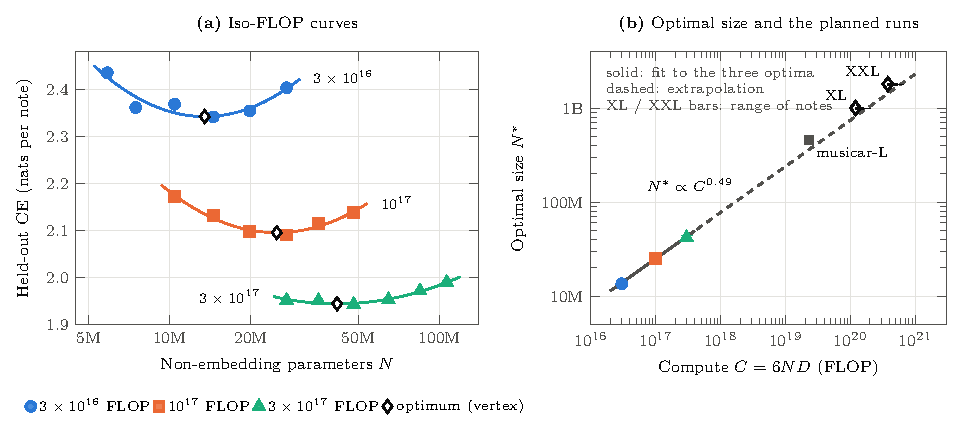
\includegraphics[width=\linewidth]{../figures/scaling_isoflop.pdf}
\caption{Iso-FLOP results on one RTX 5090. (a) Held-out CE against non-embedding parameters at three compute budgets,
a parabola in $\ln N$ per budget and its vertex. (b) Optimal size per budget (bars: bootstrap 10--90\%), the power law
through the three optima and its extrapolation; the 1B and 2B runs as planned (bars: range of notes), musicar-L as trained.
The planned sizes come from the joint fit of the loss in $N$ and $D$, which puts the optimum somewhat above this
simple line (2B at $5\times10^{20}$ FLOP; the line gives about 1.6B).}
\end{figure}

\subsubsection{Repeat penalty and model size}
Penalty = CE with repeated data $-$ CE with fresh data, same model and notes seen; 3.9 passes over 41.5M unique notes.

\begin{tabularx}{\textwidth}{|L{3.0cm}|*{6}{>{\centering\arraybackslash}X|}}
\hline
\textbf{Model} & 3M & 6M & 20M & 42M & 108M & 217M\\ \hline
\textbf{Penalty} & 0.012 & 0.082 & 0.115 & 0.133 & 0.180 & 0.233 (1 seed)\\ \hline
\end{tabularx}
\vspace{4pt}
\begin{itemize}
\item Repeated-data CE: 217M 2.560 vs 108M 2.537.
\item More unique notes at the same passes (20M, 3.86 passes): 0.115 over 41.5M vs 0.048 over 166M.
\end{itemize}
Repeating data costs more in larger models. At 3.9 passes the penalty grows from 0.012 at 3M to 0.233 at 217M, and
the 217M model ends worse than the 108M one on the same repeated data. More unique notes cut the cost: the same 20M
model at the same passes loses 0.115 over 41.5M notes and 0.048 over 166M. This is why the unique-note count matters
for runs at 1--2B.

\subsubsection{Repeat penalty and the number of passes}
\begin{itemize}
\item 6M over 41.5M unique notes, against census fresh data: 3.9 / 7.7 / 15.4 passes $\to$ 0.106 / 0.117 / 0.151 (two seeds, one at 15.4; census fresh reference, 0.082 against the replay-store fresh run).
\item Held-out CE rising during training (turn-up): 6M on 10M unique notes (0.58 parameters per note), lowest at about
23.6 passes, +0.11 by 31.5; 108M on 21M (5.1 per note), lowest at about 5.7 passes, +0.14 by 7.6. Passes limit used:
11.8.
\item 42M, 7.7 passes over 41.5M (320M notes seen) with weight decay 0.5, 4 seeds: 2.318 (2.314--2.322); weight decay
1.0 + dynamics + family at 3.9 passes (160M notes), 4 seeds: 2.480.
\end{itemize}
For a small model the penalty grows slowly with the passes, from 0.106 at 3.9 to 0.151 at 15.4. Held-out loss
started to rise only at 23.6 passes for 6M, and at 5.7 passes for 108M on a very small set (5 parameters per unique
note). We limit the planned runs to 11.8 passes, half the earliest rise at a comparable number of parameters per unique note (2B run: 0.23); the 2B run needs 4.7.

\begin{figure}[!ht]
\centering
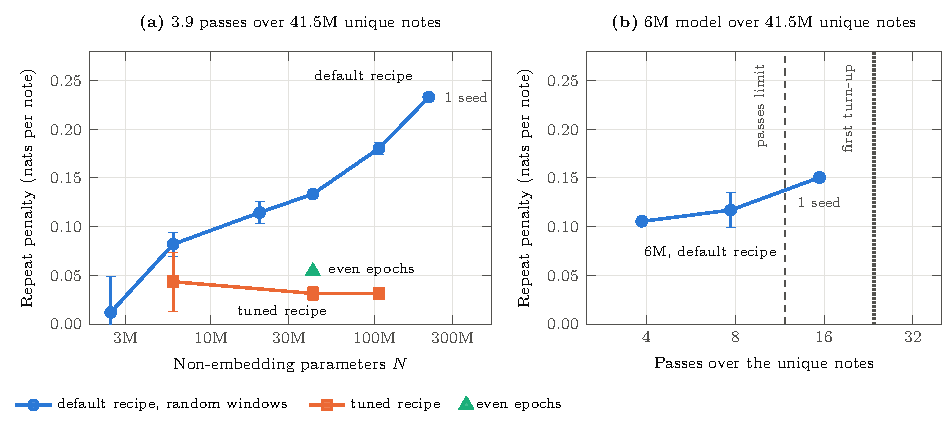
\includegraphics[width=\linewidth]{../figures/scaling_repeat.pdf}
\caption{Repeat penalty: held-out CE with repeated data minus CE with fresh data, same model and notes seen. (a)
Against model size at 3.9 passes over 41.5M unique notes: default recipe with random windows, tuned recipe (weight decay
1.0 + dynamics + instrument family), even epochs (\#26 $-$ \#24). (b) Against passes for the 6M model over the same notes.
Dashed: passes limit for the planned runs (11.8); dotted: first observed rise of held-out CE (6M on 10M unique notes, 23.6
passes). Bars: seed noise.}
\end{figure}

\subsubsection{How the data is repeated}
\begin{itemize}
\item Even epochs (\#26) vs random windows, 42M at 3.9 passes: 0.054 vs 0.134 ($\times$0.40).
\item Random-window sampler on fresh data: 2.433 vs one-pass 2.398 (\#24).
\item Census pool vs replay store, one pass, 42M: 2.387 vs 2.398.
\end{itemize}
Reading the data in even epochs instead of random windows cuts the repeat cost to 0.4$\times$ (0.054 vs 0.134 at
42M), so the planned runs read the corpus in even epochs. The census pool and the store musicar-L was trained on give
the same loss within 0.011.

\subsubsection{Predicted repeat cost for the planned runs}
Even epochs, default recipe; best-fitting form (its bootstrap 10--90\%; highest form); passes limit 11.8.

\begin{tabularx}{\textwidth}{|L{5.6cm}|L{2.4cm}|X|}
\hline
\textbf{Run} & \textbf{Passes over 8.84B} & \textbf{Penalty}\\ \hline
1B run, 20.6B notes & 2.3 & +0.001 (0.000--0.002; highest form 0.004)\\ \hline
2B run, 41.5B notes & 4.7 & +0.004 (0.002--0.007; highest form 0.032)\\ \hline
2B run at 27 notes per parameter, 54.8B & 6.2 & +0.005\\ \hline
2.5B, 50.1B notes & 5.7 & +0.005\\ \hline
\end{tabularx}
\vspace{4pt}
\begin{itemize}
\item Best size at the 2B run's budget ($5.0\times10^{20}$ FLOP) over 8.84B: 2.1--2.7B over five of the six repetition forms (Chai \& Xiong: 8.3B; best
form 2.27B, 10--90\% 2.17--2.43B); $\pm0.01$ band about 0.8--6.6B. The 2.03B shape sits inside it.
\item No repetition form passes the pre-registered leave-one-group-out check; the Chai \& Xiong form
predicts 4--8$\times$ more; all forms over-predict the even-epoch penalty 1.7--3.6$\times$ (\#26).
\end{itemize}
Over the 8.84B unique notes the best-fitting form gives almost no loss to repetition: 0.001 for the 1B run and 0.004 for
the 2B run, against 0.029 gained from 1B to 2B; only the Chai \& Xiong form (+0.032 for the 2B run) puts it at that size. All runs stay well under the 11.8-pass limit. The forms disagree at many
passes and none passes the strict leave-one-group-out check; the real cost at 1--2B is one of the things the
allocation measures.

\subsubsection{Regularisation under repetition}
42M at 3.9 passes unless noted; differences against the default recipe (weight decay 0.1).

\begin{tabularx}{\textwidth}{|L{4.6cm}|X|X|}
\hline
\textbf{Change} & \textbf{Repeated data} & \textbf{Fresh data}\\ \hline
Weight decay 0.3 & $-0.056$ & $-0.031$\\ \hline
Weight decay 1.0 & $-0.089$ (67\% of the penalty) & $-0.010$\\ \hline
Weight decay 3.0 & +0.123 & --\\ \hline
Dropout 10\% / late dropout & $-0.010$ / $-0.003$ & --\\ \hline
Embedding weight decay 0 & +0.002 & --\\ \hline
\end{tabularx}
\vspace{4pt}
\begin{itemize}
\item Tuned recipe (weight decay 1.0 + dynamics + instrument family), confirmed on new seeds ($-0.083$): CE gain over
the default 79\% of the penalty at 42M, 7.6 passes (penalty 0.509 $\to$ 0.089) and 80\% at 108M, 3.9 passes (0.181
$\to$ 0.031). Cost on fresh data:
+0.016 (42M), +0.004 (108M), +0.065 (6M).
\item One-pass iso runs at weight decay 0.3: $-0.013$ (6M), $-0.031$ (27M).
\end{itemize}
Weight decay 1.0 wins back two thirds of the repeat penalty at 42M; 3.0 is too much. Together with dynamics and
instrument-family augmentation it wins back about 80\% at 42M and 108M. On fresh data it costs a little, more for
small models. The plan is to transfer the weight decay through its decay timescale instead of copying the value,
and the WP1b search checks it.

\subsubsection{Augmentation}
\begin{itemize}
\item Against the repeated-data control (42M, 3.9 passes): dynamics $-0.026$; instrument family $-0.020$; 12 keys
$-0.004$; octave 0.000; tempo $\pm10\%$ +0.048, $\pm20\%$ +0.053.
\end{itemize}
Changing the dynamics and swapping instruments within a family help on repeated data ($-0.026$ and $-0.020$);
transposition does almost nothing and tempo changes hurt (+0.05). The tuned recipe keeps the first two.

\subsubsection{Optimiser, learning rate and batch size}
\begin{itemize}
\item Learning rate $2\times10^{-3}$ vs $10^{-3}$: repeated data 6M $-0.064$, 42M $-0.030$; fresh data 6M $-0.028$, 42M
+0.001. Iso: tilt $t = -0.018$ at $3\times10^{16}$ ($\mu$P direction), $\pm0.001$ at $10^{17}$ (\#29, \#30).
\item Batch 16,384 vs 32,768 notes (42M): repeated $-0.034$, fresh $-0.021$; at learning rate $\times$0.7 $-0.018$. Iso
batch 16,384: $-0.016$ (27M), $-0.009$ (6M).
\item NorMuon vs Muon (42M): repeated $-0.023$, fresh $-0.038$.
\end{itemize}
A higher learning rate and a smaller batch help on repeated data and less on fresh data. NorMuon beats Muon on
both by 0.02--0.04 at 42M. These settings may not transfer to 1--2B, so WP1b checks them on 6M--464M models before
the large runs.

\subsubsection{Synthetic data and distillation}
\begin{itemize}
\item musicar-L samples as 25\% of the windows: 42M 0.000, 108M $-0.016$; one synthetic note worth about 0.56--0.57
real notes.
\item Samples of a 42M model as 25\% of the windows: +0.030.
\item Distillation, 42M on repeated data: from 4 models trained on the same data $-0.073$ (54\% of the penalty), from 1
model $-0.045$; on fresh data, from 4 fresh models $-0.001$.
\end{itemize}
Samples from musicar-L are worth about 0.57 real notes each as training data, while samples from a small model
hurt. Distillation from four models trained on the same data wins back about half the repeat penalty. Both are
fallbacks if the corpus runs short, not part of the plan.

\subsubsection{Data sources}
\begin{itemize}
\item Discover stores repeat like GigaMIDI: $\rho$ 0.94 ($R^*$ 3.03 vs 3.22).
\item Aria (transcribed piano) part: $R^*$ 6.48 vs 3.03 for the whole Discover validation set ($\times$2.1).
\item A random 8.8\% file subset of the census pool at one pass: +0.060 against the full pool (6M).
\end{itemize}
The Discover MIDI part repeats almost like GigaMIDI ($\rho$ 0.94), and the transcribed piano in Aria takes about
twice as many passes before it costs the same. A random 8.8\% subset of the census pool is 0.060 worse than the full
pool at 6M.

\subsubsection{Pre-registered predictions}
\begin{tabularx}{\textwidth}{|X|L{5.2cm}|}
\hline
\textbf{Prediction (committed 21 Nov, 02:11 UTC)} & \textbf{Result}\\ \hline
Penalty at 3M: 0.13 / 0.054 / $\lesssim$0.03 (three forms) & 0.012: third form (seed noise 0.03)\\ \hline
Penalty at 217M: about 0.16 / 0.226 / equal to 108M & 0.233: second form\\ \hline
6M at 15.4 passes: 0.25--1.07 (exponential / power forms), 0.12 (Chai \& Xiong) & 0.151: closest to Chai \& Xiong, above all forms\\ \hline
Learning-rate tilt $t < 0$ at $3\times10^{16}$ & $-0.018$: yes\\ \hline
Raw notes-per-parameter bias +4--36\% at $3\times10^{16}$ & not measured (depends on an assumed offset)\\ \hline
Fresh data best at weight decay 0.2--0.4, gain 0--0.03 & 0.3, $-0.031$: yes (edge)\\ \hline
Repeated data best at weight decay $\geq$1 & 1.0: yes\\ \hline
Penalty factor $\times$0.61--0.94 at 0.3, $\times$0.19--0.61 at 1.0 & $\times$0.81, $\times$0.41: yes\\ \hline
Embedding weight decay 0 loses about 0.02 & +0.002: no\\ \hline
Fresh gain at learning rate $2\times10^{-3}$ positive, below 0.08 & 6M $-0.028$: yes; 42M +0.001: no\\ \hline
Synthetic value stays about 0.57 while the student is smaller than the teacher & 0.56--0.57, measured 20 Nov before the commit: not a test\\
\hline
\end{tabularx}
\vspace{4pt}
Of the 11 predictions written before the confirmatory runs, 5 held (3 outright, 2 by matching one of the proposed
forms), 2 held only at the edge, 2 missed (embedding weight decay and the 42M learning-rate gain on fresh data), and 2
were not tests (the synthetic value was measured before the commit; the notes-per-parameter bias depends on an assumed
offset). We report the misses as they are; the forecast
for the 1B and 2B runs is reported the same way, whether it holds or not.

\subsection{Objectives}\label{sec:objectives}
WP and D numbers refer to the work packages and development tasks in the resource table
(\seclink{sec:resources}{Section~\ref*{sec:resources}}).

\textbf{Training method}
\begin{itemize}
\item \textbf{O1 Multi-GPU trainer.} Data parallel on one 4$\times$H100 node, at least 95\% of 4$\times$ the
rate of one GPU running its 16,384-note share (the basis of the hours; the bf16 gradient all-reduce of 4.1 GB over
NVLink takes about 15--40 ms against a 0.7 s step). Then 2--4
nodes, with the efficiency measured.
\item \textbf{O2 FP8 on Hopper.} Held-out loss within 0.005 nats of a BF16 twin after 1B notes, at 1B parameters,
at the speed-up measured on the H100 (\seclink{sec:scal}{benchmark table}).
\item \textbf{O3 NorMuon at scale.} Plain data parallel repeats the Newton--Schulz step on every GPU. Sharding it over
the four GPUs (D2) should bring the 2B rate from about 22,800 to about 28,000--30,000 notes/s per GPU.
\item \textbf{O4 Hyperparameter transfer.} Learning rate, decay timescale, batch size and NorMuon settings checked on
6M--464M models, and three more iso-FLOP budgets ($10^{18}$, $3\times10^{18}$, $10^{19}$ FLOP), 30$\times$ beyond the
current fit (WP1b, 100--138 node hours).
\end{itemize}

\medskip
\textbf{Scaling runs}
\begin{itemize}
\item \textbf{O5 The 1B and 2B runs.} 1B (0.97B): 20.6--26.1B notes, $1.2$--$1.5\times10^{20}$ FLOP, 35--44 node hours.
2B (2.03B): 41.5--54.8B notes, $5.0$--$6.7\times10^{20}$ FLOP, 133--176 node hours, right after the 1B run on the
same node. Forecast: 1.570 and 1.541 nats per note; repeat cost +0.001--0.002 and +0.004--0.005 over 8.84B unique notes
(best-fitting form; no repetition form passes the leave-one-group-out check yet).
\item \textbf{O6 Evaluation.} Both runs against the forecast (it holds if the loss falls inside the 10--90\% band,
about $\pm0.035$) and against musicar-L and the open baselines: 96 continuation prompts, 96 piano prompts, English and
Ukrainian captions, CLaMP 3. A blind listening test. Paper for ISMIR 2027
(deadline expected in April) and open weights.
\end{itemize}

\medskip
\textbf{After the main runs}
\begin{itemize}
\item \textbf{O7 Ablations at 1B.} A stronger text encoder with its top layers or LoRA trained, and a context of
16,384 notes (8$\times$ now) for captions over long pieces
(\seclink{sec:encoder}{Section~\ref*{sec:encoder}}). A 2B-note continuation at 16,384 notes costs about 30--50 H100
hours (attention FLOP scaled from the measured 1B rate).
\item \textbf{O8 (optional) 2.5B.} 2.48B parameters, 50--67B notes, 205--274 node hours. The corpus supports it
(5.7--7.6 passes over 8.84B unique notes, +0.005 nats at the optimum; $7.4$--$9.9\times10^{20}$ FLOP).
\end{itemize}

\subsection{Fit with the Development Access scope}

\begin{itemize}
\item \textbf{Most of the work is development.} The trainer is single-GPU today. The project ports it to multi-GPU
and multi-node (data parallel, sharded NorMuon, FP8 on Hopper), measures the scaling from 1 to 4 GPUs and then to
2--4 nodes, and profiles the step (\seclink{sec:scal}{benchmark table}).
\item \textbf{The two runs test the method at its target scale.} The 1B and 2B runs use about a third of the request
(168--220 of 445--630 node hours); the rest is porting, the search, ablations, evaluation and reserve.
\item \textbf{Small request.} 445--630 node hours, 13--18\% of the 3,500 node hours offered per Development proposal,
over 6 months.
\item \textbf{It prepares a larger application.} The measured efficiency, the scaling law at 1--2B and the repeat cost
are the numbers an AI Factory or Regular Access proposal needs, for larger models, longer contexts or encoder
training.
\item \textbf{Open results.} Code, weights, logs and the forecast against the measured loss are released, so other
groups can use the scaling law and the repeat cost without repeating the runs.
\end{itemize}

\subsection{Text encoder and captions over long contexts}\label{sec:encoder}

\textbf{Current encoder}
\begin{itemize}
\item \textbf{LaBSE} (\texttt{sentence-transformers/LaBSE}), frozen: 471M parameters, of which about 385M are the
vocabulary table; the transformer is BERT-base (12 layers, width 768). Chosen in October because it matched every
Ukrainian prompt to its English translation (20/20; multilingual-e5-small 12/20, e5-base 10/20).
\item Its token states go through a trained adapter (16 learned queries, one attention layer and a 2-layer MLP;
12.6M parameters with the section adapter) into 16 file-caption vectors in front of the notes and 4 section-caption
vectors where each section caption arrives, through a gate initialised at 0.01 (zero gave NaN gradients).
\item It is too weak for long prose: on MidiCaps captions musicar-L-caption comes last, with the key match at the
shuffled baseline.
\end{itemize}

\medskip
\textbf{Possible replacements} (all multilingual, so Ukrainian prompts keep working)
\begin{itemize}
\item \textbf{CLaMP 3 text encoder} (XLM-RoBERTa base): trained contrastively on music--text pairs, including
symbolic music, so its space is already aligned with music; trained on text of up to 128 tokens.
\item \textbf{BGE-M3} (568M, XLM-RoBERTa large): inputs up to 8,192 tokens, strong on long multilingual text.
\item \textbf{Qwen3-Embedding} (0.6B or 4B): inputs up to 32K tokens, among the strongest multilingual embedders.
\item \textbf{multilingual-e5-large} (560M): a larger version of the encoder that lost to LaBSE at small size.
\item \textbf{jina-embeddings-v3} (570M, 8,192 tokens): strong, but its licence is non-commercial.
\item \textbf{A small LLM's hidden states} (Llama 3.2 1B, as MIDI-LLM uses, or Qwen 1.7B): the richest reading of
long captions, and the slowest.
\end{itemize}

\medskip
\textbf{What needs training}
\begin{itemize}
\item Always: the caption adapter (13M now, 15--21M at the 1--2B widths; its input width changes from 768 to 1,024 for most of the
encoders above) and the caption and section vectors.
\item Ablation: LoRA on the encoder (a few M parameters) or its top 2--4 layers (about 25--50M on a 0.5B encoder).
The encoder reads only the caption, so its cost is small next to the 1--2B trunk.
\item For long contexts: section captions at every section of a 16,384-note window, through the section slots or the
cross-attention every two blocks that the code already has, trained on windows that span several sections.
\end{itemize}

\medskip
\textbf{Captions for long pieces}
\begin{itemize}
\item Long-context training needs a caption for every section, not one per file. Part of them will be written by
\textbf{Claude Haiku 5.5} (Anthropic) from features computed from the MIDI (tempo, key, instruments, density, section
boundaries) and the file metadata, in English and Ukrainian. The rest come from the template captions built from
metadata, MidiCaps and the XMIDI labels.
\item This is also a \textbf{self-improvement loop} worth studying on its own: musicar generates pieces, a language
model describes them, and the caption--piece pairs train the next model to follow text. As plain training data,
musicar-L samples were worth about 0.57 real notes each (Section~\ref{sec:prelim}); whether captioned samples help
caption following is tested in the ablation.
\end{itemize}

\medskip
\textbf{The open question}
\begin{itemize}
\item We know of no published method that makes a music model follow captions over a long piece. In our runs the caption's
influence fades as the piece goes on, and switching at section changes is only partial.
\item With a trained encoder, a 16K context and enough compute, a few test runs can answer it: which encoder, what to
train, where the captions go. The RTX 5090 budget did not allow testing these hypotheses; the allocation does.
\end{itemize}
\section{Partitions and resource request}\label{sec:partitions}
\subsection{Partition choice}
\begin{itemize}
\item 4$\times$H100 nodes preferred: the code was developed and trained on CUDA GPUs (RTX 5090), the FP8 path uses
Hopper / Blackwell tensor cores, and the H100 benchmark (Section~\ref{sec:scal}) was measured on an H100 SXM 80 GB capped at 64 GB (same
generation; MN5's 64 GB card may have less memory bandwidth, which the cap does not model).
\item Jobs: the EuroHPC queue \texttt{acc\_ehpc} allows 72 h per job and up to 100 nodes. The 1B run (34--45 h on one
node) fits in one job, the 2B run (133--176 h) in two or three, each resuming from a checkpoint; queue waits are not
published.
\end{itemize}
\begin{tabularx}{\textwidth}{|L{3.0cm}|L{3.0cm}|X|}
\hline
\textbf{Partition} & \textbf{Node} & \textbf{Notes}\\ \hline
MareNostrum 5 ACC & 4$\times$ H100 64 GB & Chosen. FP8 works; in the call's systems table (Oct 2026) with 3,500
node hours for Development\\ \hline
JUPITER Booster & 4$\times$ GH200 96 GB & Not requested (H100 chosen); ARM host CPU (aarch64 wheels, container);
3,500 node hours\\ \hline
Leonardo Booster & 4$\times$ A100 64 GB & Fallback only. No FP8, so BF16 and more hours; 4,500 node hours\\ \hline
LUMI-G & AMD MI250X & ROCm port; not planned\\ \hline
\end{tabularx}
\vspace{4pt}

\subsection{Resource estimate}\label{sec:resources}
\begin{tabularx}{\textwidth}{|L{5.0cm}|L{2.3cm}|L{2.2cm}|X|}
\hline
\textbf{Work package} & \textbf{H100 hours} & \textbf{Node hours} & \textbf{Basis}\\ \hline
WP1 port, scaling tests, benchmarks. For the paper runs (one node): D1 data parallel (torchrun); D2 NorMuon step
sharded over the 4 GPUs (before WP3, saves about 25\% of its hours); D3 FP8 checked against BF16, fused FP8 casts; D5
data loading from memory-mapped stores on the parallel file system; D6 checkpoint and restart under the 72 h limit (the trainer already saves a resumable checkpoint on SIGTERM); D7
evaluation pipeline on the cluster. Later: D4 sharding (FSDP / ZeRO), D8 multi-node launch and scaling to 8--64 GPUs
& 300--500 & 75--125 & one node first, then scaling curves 1--64 GPUs\\ \hline
WP1b hyperparameter search and scaling points (6M--464M; iso-FLOP $10^{18}$--$10^{19}$) & 400--550 & 100--138 &
4 single-GPU runs packed per node\\ \hline
WP2 1B run (28$\times$1664), 20.6--26.1B notes & 138--175 & 35--44 & 43,600 notes/s per GPU measured;
1.4--1.8 days on one node\\ \hline
WP3 2B run (37$\times$2112), 41--55B notes, right after WP2 & 530--700 & 133--176 & 22,800 notes/s per GPU
(24,900 measured for 36$\times$2048, scaled by parameters); 5.5--7.3 days on one node\\ \hline
WP4 ablations at 1B after the 2B run (text encoder, context 16,384) & 150--200 & 38--50 & RTX 5090-based estimate\\ \hline
WP5 evaluation & 30--50 & 8--13 & head-to-head, CLaMP 3\\ \hline
Reserve for restarts (15\%) & 230--330 & 58--82 & \\ \hline
\textbf{Total} & \textbf{1,780--2,500} & \textbf{445--630} & 13--18\% of the 3,500 node-hour offer\\ \hline
WP6 (optional) 2.5B (38$\times$2304), 50--67B notes & 820--1,095 & 205--274 & 17,900 notes/s per GPU measured;
8.5--11.4 days on one node; not in the total\\ \hline
\end{tabularx}
\vspace{4pt}

\begin{itemize}
\item Notes per run: the lower end is the optimum of the fitted law (about 21 notes per parameter), the upper end
27 notes per parameter (the per-budget optima drift up to about 32); WP1b fixes the choice before WP2.
\item The two main runs need 168--220 node hours, 7--9 days on one node; the whole request is 19--26 days of one
node; with the optional 2.5B and its 15\% reserve, 2,720--3,760 H100 hours (680--945 node hours, 19--27\% of the offer).
\item Hours of WP2, WP3, WP6 = notes / the notes/s measured (for WP3 scaled from 36$\times$2048 to 37$\times$2112 by the
parameter count, 1.09$\times$; a short H100 run before the award would replace the estimate) on one H100 SXM 80 GB at one GPU's share of a 65,536-note
step with 4-GPU data parallel (FP8, Muon, 64 GB cap; includes the redundant Muon update) / 0.95 for the all-reduce;
node hours = H100 hours / 4. With D2 the runs need about 25\% less (WP2 104--131, WP3 400--530 H100 hours). WP1b
and WP4 keep the RTX 5090-based estimate (conservative: the H100 measured 1.69$\times$ the RTX 5090).
\end{itemize}

\subsection{Memory}
\begin{itemize}
\item All planned shapes fit the 64 GB of an MN5 ACC H100 without sharding (peaks in the benchmark table,
Section~\ref{sec:scal}); data parallel is enough for the paper runs.
\end{itemize}

\subsection{Storage and I/O}
\begin{itemize}
\item Full stores for 21--26B / 41--55B notes seen (one copy of the corpus, read in even epochs): 89.7 GB for all
9.92B notes (9 bytes per note), about 80 GB for the 8.84B left after near-duplicate removal at Jaccard 0.8.
\item Checkpoints: bf16 weights about 2 GB (1B) and 4.1 GB (2B); full resumable state about 6 GB and 12.5 GB by
parameter count (fp32 weights, optimiser states).
\item Data loader read rate: about 1.6 MB/s per node at the 1B rate (174,000 notes/s, 9 bytes per note), small for a
parallel file system.
\end{itemize}

\subsection{Data transfer}
\begin{itemize}
\item In: token stores from the private Hugging Face dataset repository or by scp; volume as above.
\item Out: final weights and logs to Hugging Face; evaluation outputs.
\end{itemize}

\section{Code details, development and feasibility}\label{sec:code}
\subsection{Software and libraries}
\begin{itemize}
\item Python 3.12, PyTorch 2.14 (CUDA 13.0 wheels), torchao 0.18 (float8), torch.compile, transformers (frozen
LaBSE), wandb optional.
\item Own code: model, trainer, Muon (8-bit AdamW from torchao), data stores, evaluation harness (GitHub).
\item Environment on the cluster: a Singularity container (MN5 module \texttt{singularity}, run with
\texttt{singularity exec --nv}) holding the same PyTorch / CUDA 13 stack as on the RTX 5090. The node
driver must support CUDA 13 (driver 580 or newer); with an older driver the container uses a CUDA 12.8 build.
\end{itemize}

\subsection{Training setup}\label{sec:setup}
Setup of the 1B and 2B runs. ``Search'' = fixed by the WP1b search on 6M--464M models before the runs.

\begin{tabularx}{\textwidth}{|L{3.4cm}|X|L{2.6cm}|}
\hline
\textbf{Item} & \textbf{Setting} & \textbf{Found in search}\\ \hline
Model & Decoder-only transformer as musicar-L: compound note tokens, cascade output heads, RMSNorm, QK-norm, RoPE,
SwiGLU & no\\ \hline
Shapes & 1B: 28 blocks $\times$ 1664 (26 heads); 2B: 37 $\times$ 2112 (33 heads); head size 64 & no\\ \hline
Context & 2,048 notes (16,384 in the WP4 ablation) & no\\ \hline
Loss & Teacher-forced sum of five cross-entropies (time shift, instrument, pitch, duration, velocity); reported losses sum the four note attributes & no\\ \hline
Optimiser & NorMuon on the block matrices, AdamW on embeddings, heads and norms (NorMuon beat Muon by 0.023 on
repeated and 0.038 on fresh data at 42M) & no; its settings yes\\ \hline
Learning rate & musicar-L used $10^{-3}$; the value for 1--2B and its scaling with width & yes\\ \hline
Schedule & Warmup--stable--decay; length of the decay & decay length yes\\ \hline
Weight decay & Transferred through the decay timescale, not copied; 0.3 was best on fresh and 1.0 on repeated data at
42M & yes\\ \hline
Batch & 65,536 notes per step in the benchmark; 16,384 was better at 42M & yes\\ \hline
Notes per parameter & 20.4 (fitted optimum) to 27: 1B run 20.6--26.1B, 2B run 41.5--54.8B notes & yes\\ \hline
Precision & bf16 autocast with FP8 matrix multiplies (torchao), torch.compile; checked against BF16 (D3) & no\\ \hline
Data & Census stores, 8.84B unique notes after near-duplicate removal, read in even epochs & no\\ \hline
Augmentation & Dynamics and instrument-family swaps on; no tempo change & no\\ \hline
Micro-batch, checkpointing & Per partition, by the preflight micro-batch search & preflight\\ \hline
Parallelism & Data parallel on one 4-GPU node; NorMuon step sharded (D2); gradient all-reduce of 4.1 GB (2B, bf16 hook;
8.1 GB in fp32) over NVLink, about 15--40 ms against a 0.7 s step & no\\ \hline
Evaluation & Held-out loss during the run; a cooldown can branch from an earlier checkpoint if it rises & no\\ \hline
\end{tabularx}
\vspace{4pt}

\subsection{Current state of the code}
\begin{itemize}
\item Single GPU only: train.py has no DDP / FSDP / torchrun path. This is the main development item.
\item Existing tooling to reuse: preflight (benchmark, micro-batch search, LR probe, smoke tests), resumable runs,
OOM recovery, checkpoint sync, the scaling-sweep and fit tools (\path{tools/sweeps}).
\item To replace on the cluster: Hugging Face Hub sync by the parallel file system; vast.ai scripts by Slurm job
scripts.
\end{itemize}

\subsection{Benchmarks}\label{sec:scal}
One rented H100 SXM 80 GB (700 W), 22 Nov 2026: synthetic batches, Muon, torch.compile, memory capped at 64 GB to match
MN5 ACC. Rates in notes per second per GPU.

\begin{tabularx}{\textwidth}{|L{3.8cm}|X|}
\hline
\textbf{Measurement} & \textbf{Result}\\ \hline
H100 against RTX 5090 & musicar-L, FP8, best micro-batch on each (16 vs 8): 95,339 vs 56,468 notes/s (1.69$\times$)\\ \hline
Rate per GPU: full 65,536-note step / one GPU's share of a 4-GPU step (FP8) & 1B (28$\times$1664) 58,055 / 43,599;
1.87B (36$\times$2048) 32,894 / 24,904; 2.5B (38$\times$2304) 25,627 / 17,876. The final 2B (37$\times$2112) was not run:
about 30,100 / 22,800 by scaling with the parameter count\\ \hline
Peak memory (64 GB cap) & 1B 22--58 GB (30 GB in the 4-GPU-share setup used for the hours); 1.87B 35--39 GB for the
full step (micro-batch 4, or 16 with full activation checkpointing) and 49 GB in the 4-GPU-share setup; 2.5B 43--46
GB; final 2B about 50--53 GB in the 4-GPU-share setup by scaling\\ \hline
Repeated Newton--Schulz step under plain data parallel & $-25\%$ at 1B and 1.87B, $-30\%$ at 2.5B; removed by D2\\
\hline
FP8 against BF16 & $-6\%$ at musicar-L's width, $+7\%$ at 1B, $+10\%$ at 1.87B\\ \hline
Step profile, 1.87B & forward 24\%, backward 62\%, optimiser 13\% of the time; kernels: FP8 scaling and casts 39\%,
matrix multiplies 36\%, elementwise 13\%, attention 12\%\\ \hline
Other options & caching FP8 weights per step 0--2\%; wider shapes of the same size +3\% (1B) and +7\% (1.87B)\\ \hline
RTX 5090 & musicar-L with FP8 56,468 notes/s against 44,230 in BF16 ($+28\%$)\\ \hline
Next speed-ups & fused FP8 casts (the largest share left); sharded NorMuon step (D2); overlap of the all-reduce with
the backward pass; micro-batch search per partition\\ \hline
To measure on MN5 & scaling 1 $\to$ 4 GPUs on one node, then 2--4 nodes; all-reduce cost in the real setup\\ \hline
\end{tabularx}
\vspace{4pt}

\section{Data management}\label{sec:data}
\begin{itemize}
\item \textbf{Training data}: the census token stores, 9.92B notes after removing copies (same bytes, same tokens or the same notes) and 8.84B after
near-duplicate removal, from seven open corpora. Licences: GigaMIDI CC BY-NC 4.0; Discover MIDI, Aria-MIDI and
PianoCoRe CC BY-NC-SA 4.0; PIAST and IrishMAN MIT; BEAT has no stated licence and can be left out (8.73B unique notes
without it). The stores hold tokens only, no raw MIDI.
\item \textbf{Captions}: MidiCaps captions (CC BY-SA 4.0) and XMIDI emotion and genre labels (no licence stated,
research only); section captions partly written by Claude Haiku 5.5 from MIDI features and metadata, no audio.
No audio-derived Ukrainian song data in pretraining; Ukrainian captions are text only.
\item \textbf{No redistribution of data}: the stores move to the cluster from a private Hugging Face dataset
repository and stay on the project file system.
\item \textbf{Outputs}: weights and logs under CC BY-NC-SA 4.0 on Hugging Face, following the non-commercial
training data; code on GitHub.
\end{itemize}

\section{Expected outputs and dissemination}\label{sec:outputs}
\begin{itemize}
\item Weights, code and training logs of every run; model cards naming EuroHPC and the system.
\item The forecast against the measured loss, published whether it holds or not. Committed before the runs: fresh-data
held-out loss 1.570 for the 1B run and 1.546 for the 2B as first planned (1.8B, 35B notes); refitted for the final
shapes on 23 Nov: 1.541 for the 2.03B at 41.5B notes, 10--90\% band about $\pm0.035$; repeat cost +0.004 (10--90\%
0.002--0.007) over 8.84B unique notes.
\item A scaling-law paper on MIDI (compute-optimal notes per parameter, the cost of repeated data) with the 5090
runs and the EuroHPC runs as its out-of-sample test; target ISMIR 2027 with both runs (deadline expected around April
2027).
\item Head-to-head tables rerun with the new models; blind listening test page.
\item arXiv paper with TalTech affiliation and EuroHPC acknowledgement.
\end{itemize}

\appendix
\section{Where the results are}
Where each result in this document can be checked. Paths are in the public repository
\url{https://github.com/DmytroHilei/Music_generative_model}.

\begin{longtable}{|L{5.0cm}|L{9.6cm}|}
\hline
\textbf{Result} & \textbf{Where}\\ \hline
\endhead
musicar-L: size, shape, training, validation loss & \path{docs/model_cards/musicar-L.md};
\url{https://huggingface.co/Dimitri-206265/musicar-L}\\ \hline
musicar-L-caption: fine-tuning stages, encoder, length control & \path{docs/model_cards/musicar-L-caption.md};
\url{https://huggingface.co/Dimitri-206265/musicar-L-caption}\\ \hline
Head-to-head summary (continuation, piano, captions, MidiCaps) & \path{README.md}, head-to-head section\\ \hline
Continuation, 96 prompts: D and bootstrap & \path{docs/head2head/scores_96.md}, \path{docs/head2head/bootstrap_cont96.md}\\ \hline
Continuation, CLaMP 3 (1,000 / 200 notes) & \path{docs/head2head/cont96_clamp3_n1000.md}, \path{docs/head2head/cont96_clamp3_n200.md}\\ \hline
Solo piano, D and CLaMP 3 & \path{docs/head2head/bootstrap_piano96.md}, \path{docs/head2head/piano96_clamp3_n1000.md},
\path{docs/head2head/piano96_clamp3_n200.md}\\ \hline
Captions (our 28 prompts) & \path{docs/head2head/scores.md}, \path{docs/head2head/text_clamp3.md}\\ \hline
MidiCaps (495 captions) & \path{docs/head2head/midicaps_scores.md}, \path{docs/head2head/midicaps_clamp3.md}\\ \hline
Pre-registered predictions (21 Nov) & \path{docs/scaling/predictions_2026-11-21.md}\\ \hline
Iso-FLOP runs & \path{docs/scaling/isoflop_runs_2026-11-22.json}\\ \hline
Fresh-data law, repetition forms, request table & \path{docs/scaling/frontier_report_2026-11-22.md} (committed fit),
\path{docs/scaling/frontier_report_2026-11-23.md} (refit for the final shapes)\\ \hline
Scaling figures and their data & \path{docs/figures/scaling_isoflop.pdf}, \path{docs/figures/scaling_repeat.pdf},
\path{docs/figures/scaling_data/}\\ \hline
Fit code & \path{tools/sweeps/isoflop_fit.py}, \path{tools/sweeps/frontier_fit.py}, \path{tools/sweeps/scaling_figs.py}\\ \hline
H100 benchmark & \path{docs/scaling/h100_bench_2026-11-22/bench.md}\\ \hline
Unique notes (full MinHash pass) & \path{docs/scaling/minhash_full_2026-11-23.json}; code
\path{data_prep/census/minhash_full.py}\\ \hline
Model and trainer code & \path{musicar/}, \path{train.py}\\ \hline
\end{longtable}

\section*{References}
\textbf{Models and benchmarks}
\begin{enumerate}[label={[\arabic*]},nosep,leftmargin=2.2em]
\item J. Thickstun et al., Anticipatory Music Transformer, TMLR 2024, arXiv:2306.08620.
\item Z. Guo, S. Dixon, Moonbeam: a MIDI foundation model using both absolute and relative music attributes,
arXiv:2505.15559.
\item SkyTNT, midi-model tv2o-medium, \url{https://huggingface.co/skytnt/midi-model-tv2o-medium}.
\item X. Qu et al., MuPT: a generative symbolic music pretrained transformer, ICLR 2025, arXiv:2404.06393.
\item R. Yuan et al., ChatMusician: understanding and generating music intrinsically with LLM, arXiv:2402.16153.
\item S.-L. Wu et al., MIDI-LLM: improving text-to-MIDI music generation via adapting large language models,
arXiv:2511.03942.
\item K. Bhandari et al., Text2midi: generating symbolic music from captions, AAAI 2025, arXiv:2412.16526.
\item S. Wu et al., CLaMP 3: universal music information retrieval across unaligned modalities and unseen
languages, arXiv:2502.10362.
\setcounter{refc}{\value{enumi}}
\end{enumerate}

\textbf{Data}
\begin{enumerate}[label={[\arabic*]},nosep,leftmargin=2.2em]
\setcounter{enumi}{\value{refc}}
\item K. J. M. Lee et al., The GigaMIDI dataset with features for expressive music performance detection,
arXiv:2502.17726.
\item Project Los Angeles, Discover MIDI dataset,
\url{https://huggingface.co/datasets/projectlosangeles/Discover-MIDI-Dataset}.
\item L. Bradshaw, S. Colton, Aria-MIDI: a dataset of piano MIDI files for symbolic music modeling, ICLR 2025,
arXiv:2504.15071.
\item I. Borovik, PianoCoRe: combined and refined piano MIDI dataset, TISMIR, arXiv:2605.06627.
\item H. Bang et al., PIAST: a multimodal piano dataset with audio, symbolic and text, arXiv:2411.02551.
\item L. Qian et al., BEAT: tokenizing and generating symbolic music by uniform temporal steps, arXiv:2604.19532.
\item S. Wu et al., TunesFormer: forming Irish tunes with control codes by bar patching (IrishMAN),
arXiv:2301.02884.
\item J. Melechovsky et al., MidiCaps: a large-scale MIDI dataset with text captions, ISMIR 2024, arXiv:2406.02255.
\item S. Tian et al., XMusic: towards a generalized and controllable symbolic music generation framework (XMIDI),
arXiv:2501.08809.
\setcounter{refc}{\value{enumi}}
\end{enumerate}

\textbf{Scaling and training}
\begin{enumerate}[label={[\arabic*]},nosep,leftmargin=2.2em]
\setcounter{enumi}{\value{refc}}
\item J. Hoffmann et al., Training compute-optimal large language models, NeurIPS 2022, arXiv:2203.15556.
\item N. Muennighoff et al., Scaling data-constrained language models, NeurIPS 2023, arXiv:2305.16264.
\item J. Liu et al., Muon is scalable for LLM training (Moonlight), arXiv:2502.16982.
\item Z. Li et al., NorMuon: making Muon more efficient and scalable, arXiv:2510.05491.
\setcounter{refc}{\value{enumi}}
\end{enumerate}

\textbf{Text encoders}
\begin{enumerate}[label={[\arabic*]},nosep,leftmargin=2.2em]
\setcounter{enumi}{\value{refc}}
\item Anthropic, Claude Haiku 5.5 (\texttt{claude-haiku-5-5}), \url{https://www.anthropic.com/claude/haiku}.
\item F. Feng et al., Language-agnostic BERT sentence embedding (LaBSE), ACL 2022, arXiv:2007.01852.
\item J. Chen et al., M3-Embedding (BGE-M3), arXiv:2402.03216.
\item L. Wang et al., Multilingual E5 text embeddings: a technical report, arXiv:2402.05672.
\item S. Sturua et al., jina-embeddings-v3: multilingual embeddings with task LoRA, arXiv:2409.10173.
\item Y. Zhang et al., Qwen3 Embedding: advancing text embedding and reranking through foundation models,
arXiv:2506.05176.
\setcounter{refc}{\value{enumi}}
\end{enumerate}

\textbf{This project}
\begin{enumerate}[label={[\arabic*]},nosep,leftmargin=2.2em]
\setcounter{enumi}{\value{refc}}
\item D. Hilei, musicar code and models:\newline \url{https://github.com/DmytroHilei/Music_generative_model},\newline
\url{https://huggingface.co/Dimitri-206265}.
\end{enumerate}

\end{document}
